\documentclass[12pt, twoside]{article}
\usepackage[letterpaper, margin=1in, headsep=0.2in]{geometry}
\setlength{\headheight}{0.6in}
%\usepackage[english]{babel}
\usepackage[utf8]{inputenc}
\usepackage{microtype}
\usepackage{amsmath}
\usepackage{amssymb}
%\usepackage{amsfonts}
\usepackage{siunitx} %units in math. eg 20\milli\meter
\usepackage{yhmath} % for arcs, overparenth command
\usepackage{tikz} %graphics
\usetikzlibrary{quotes, angles}
\usepackage{graphicx} %consider setting \graphicspath{{images/}}
\usepackage{parskip} %no paragraph indent
\usepackage{enumitem}
\usepackage{multicol}
\usepackage{venndiagram}

\usepackage{fancyhdr}
\pagestyle{fancy}
\fancyhf{}
\renewcommand{\headrulewidth}{0pt} % disable the underline of the header
\raggedbottom
\hfuzz=2mm %suppresses overfull box warnings

\usepackage{hyperref}

\fancyhead[LE]{\thepage}
\fancyhead[RO]{\thepage \\ Name: \hspace{4cm} \,\\}
\fancyhead[LO]{BECA / Dr. Huson / Geometry\\*  Unit 2: Angles\\* 28 Sept 2022}

\begin{document}

\subsubsection*{2.1 Classwork: Angle measures}
\begin{enumerate}
\item Use the image of the protractor to measure each of the angles. \par \medskip
  \begin{tikzpicture}
    \draw[thick] (-3,0)--(0,0)--(3,0);
    \draw (4,0) arc (0:180:4);
    \draw[thick] (0,0) circle [radius=0.1];
    \foreach \x in {0,15,30,...,180}
      \node at (\x:3.4){\x};
    \foreach \x in {0,15,30,...,180}
      \draw (\x:3.7)--(\x:4);
    \foreach \x in {0,5,...,180}
      \draw (\x:3.9)--(\x:4);
    \draw[->,thick] (0,0)--(25:4.5)node[right]{$m\angle A = \rule{2cm}{0.1mm}$};
    \draw[->,thick] (0,0)--(68:4.5)node[right]{$m\angle B = \rule{2cm}{0.1mm}$};
    \draw[->,thick] (0,0)--(125:4.5)node[left]{$m\angle C = \rule{2cm}{0.1mm}$};
  \end{tikzpicture}

\item
\begin{enumerate}
  \item Write down the name of the angle below using proper geometric notation.
  \item Find the measure of the angle in degrees with a protractor.
  \item Is it an acute, obtuse, or right angle?
\end{enumerate}
    \begin{flushright}
    \begin{tikzpicture}[scale=2]
      \draw [->, thick] (0,0)--(40:4);
      \draw [->, thick] (0,0)--(-20:5);
      \draw [fill] (40:3) circle [radius=0.025] node[above left ]{$D$};
      \draw [fill] (0,0) circle [radius=0.025] node[above left]{$E$};
      \draw [fill] (-20:4) circle [radius=0.025] node[above]{$F$};
    \end{tikzpicture}
    \end{flushright}

\item Circle True or False for each statement.
\begin{multicols*}{2}
  \begin{enumerate}
    \item T \quad F \quad Point $P$ is the vertex
    \item T \quad F \quad $\overrightarrow{OP}$, $\overrightarrow{OS}$ are opposite rays
    \item T \quad F \quad m$\angle ROS = 90^\circ$
    \item T \quad F \quad $\angle QOS$ is an acute angle
  \end{enumerate}
  \begin{tikzpicture}[scale=0.8, rotate=0]
    \draw [->, thick] (0,0)--(129:4);
    \draw [<->, thick] (-4,0)--(3,0)node[below]{$S$};
    \draw [->, thick] (0,0)--(0,4);
    \draw (0,0)++(0.4,0)--++(0,0.4)--+(-0.4,0);
    \draw [fill] (129:3) circle [radius=0.05] node[below left]{$Q$};
    \draw [fill] (-3,0) circle [radius=0.05] node[below]{$P$}; 
    \draw [fill] (0,0) circle [radius=0.05] node[below right]{$O$};
    \draw [fill] (0,3) circle [radius=0.05] node[right]{$R$};
    %\node at (-1,0.4){$51^\circ$};
    %\node at (-0.4,1.2){$x^\circ$};
  \end{tikzpicture}
\end{multicols*}

\newpage
\item Using the given ray $\overrightarrow{AB}$ as one leg, draw an angle that measures $55^\circ$. \par \vspace{5cm} \hspace{3cm}
  \tikz{
    \draw [->, thick] (0,0)--(0:8)node[below left]{$B$};
    \fill (0,0) circle [radius=0.07cm]node[below]{$A$};}

 
\end{enumerate}
\end{document}